\section{Methods and materials}
\subsection{Introduction}
System Overview The aim of this paper is to introduce a Direct Current (DC) microgrid Energy Management System (EMS) utilizing system of systems (SOSs). The proposed system involves the integration of renewable energy sources, energy storage, and demand management within a microgrid framework. The Matlab Simulink environment is employed to model and simulate the system.
\subsection{Microgrid configuration}
The microgrid comprises four houses, each symbolizing a unique scenario. As depicted in Figure 4.1, these houses are interconnected with the Central Grid Management System (CGMS) via a microgrid. In the Matlab Simulink model, each house is represented as a distinct block
\begin{figure}[H]
	\centering
	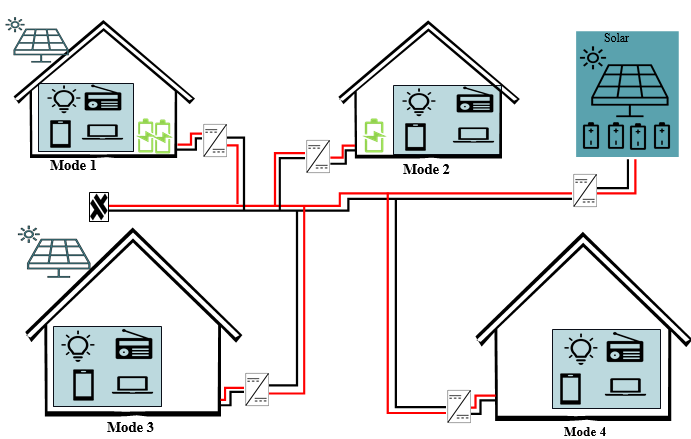
\includegraphics[totalheight=8cm]{Figures/re dc mg1.png}
	\caption{Residential unit operation modes.}
	%	\label{fig:verticalcell}
\end{figure}
\subsection{Scenarios for diverse inputs}
The four houses in the microgrid allow for the simulation of various scenarios that serve as input parameters for the CGMS:

\begin{list}{}{}
%	\setlength\itemsep{-1em}
	\item Scenario 1: Node with Storage System In this scenario, a node within the microgrid is equipped with an energy storage system. This system can both store and source energy, providing flexibility in managing energy demand and supply.\par
	\item Scenario 2: Node without Storage System This scenario involves a node that lacks an energy storage system. Energy can only be sourced from renewable sources (e.g., solar panels) during periods of sunlight.\par
	\item Scenario 3: Node with Only Storage System Here, a node in the microgrid is equipped with an energy storage system but does not possess the capability to generate energy. It can only manage energy based on stored reserves.\par
	\item Scenario 4: System Node with No Energy Interaction This scenario represents a node in the microgrid that neither stores nor sources energy. It serves to demonstrate the impact of non-participating nodes on the overall energy management system.\par
\end{list}

\section{Matlab Simulink Model}
The proposed microgrid EMS and scenarios are implemented using the Matlab Simulink platform. Each scenario is modeled as a separate block, with appropriate connections to represent energy flow, storage, and interaction with the microgrid.\par
\section{Validation and Verification}
The proposed microgrid EMS's validity is confirmed by conducting comparisons with a laboratory model and benchmark scenarios. Sensitivity analysis is conducted to assess the system's robustness to varying parameters.\par
\section{Microgrid Formation}
By combining these individual house blocks, a comprehensive microgrid is formed. This microgrid is integrated with the CGMS, allowing for centralized energy management and coordination across the various scenarios. In the absence of CGMS, the microgrid can still operate under systems of systems rule. The formation of a microgrid involves the integration of four distinct units, each of which presents a unique scenario for analysing the response of the energy management system.
\subsection{Photo Voltaic Solar Panels}
In the evaluation of the system, two series of interconnected PV modules with parameters as specified in Table 4.1 are employed. The output voltage and current of these PV modules are calculated by applying irradiance and temperature data sourced from \cite{41}, utilizing the following equation:
\begin{equation}
	{I_d}={I_o}(\exp(\frac{{V_d}}{{V_T}})-1)
\end{equation}
\begin{equation}
	{V_T}=\frac{{k_t}}{{q}}*nl*NCell
\end{equation}

\begin{center}
	\begin{table}[!ht]
		\begin{center}
			\caption{PV array parameters}
			%\label{tab:table1}
			\begin{tabular}{|p{6cm}|p{4cm}|p{4cm}|} % <-- Alignments: 1st column left, 2nd middle and 3rd right, with vertical lines in between
				\hline
				\textbf{Parameter (Unit)} & \textbf{Solar Farm PV} & \textbf{Solar Farm PV}\\
				\hline
				Maximum Power(W) & 330 & 330\\
				\hline
				Open circuit voltage(V) & 36.84 & 48\\
				\hline
				Short-circuit current Isc (A) & 100 & 19.896\\
				\hline
				Voltage at maximum power point Imp (V) & 100 & 22\\
				\hline
				Current at maximum power point Imp (A) & 55.87 & 55.87\\
				\hline
			\end{tabular}
		\end{center}
	\end{table}
\end{center}

Figure 4.6.1 displays the irradiance and temperature data intended for use as input parameters in the PV simulation block. Given their close proximity, it can be inferred that the irradiance will be consistent across all units
\begin{figure}[H]
	\centering
	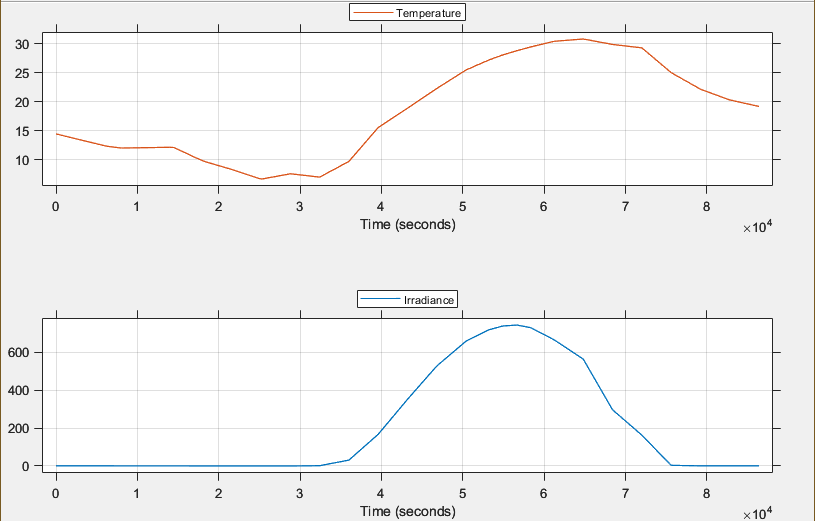
\includegraphics[totalheight=8cm]{Figures/irradiance.png}
	\caption{Photo Voltaic Generation Irradiance and Temperature 8/16/2020\cite{41}}
	%	\label{fig:verticalcell}
\end{figure}
The battery's capacity rating, as illustrated in Table 4.2. Shows two battery capacities used in this paper, The solar farm energy storage system (SF ESS) and Residential energy storage system (RE BSS). The Solar farm battery storage boasts a substantial maximum capacity of 100 ampere-hours (Ah), enabling it to store a significant amount of electric charge. With a nominal voltage of 48 volts (V), SF ESS maintains a consistent grid operating voltage while it is charged. RE BSS is a specialized energy storage solution operated by a REMCS in a MG, it is designed to complement SF ESS.

\begin{center}
	\begin{table}[!ht]
		\begin{center}
			\caption{Energy storage parameters}
			%\label{tab:table1}
			\begin{tabular}{|p{6cm}|p{4cm}|p{4cm}|} % <-- Alignments: 1st column left, 2nd middle and 3rd right, with vertical lines in between
				\hline
				\textbf{Parameter (Unit)} & \textbf{SF ESS} & \textbf{RE BSS}\\
				\hline
				Maximum capacity (Ah) & 100 & 22\\
				\hline
				Nominal voltage(V) & 48 & 48\\
				\hline
				Nominal capacity (Ah) & 100 & 19.896\\
				\hline
				Rated capacity (Ah) & 100 & 22\\
				\hline
				Fully Charged Voltage (V) & 55.87 & 55.87\\
				\hline
				Cut-off voltage (V) & 36 & 36\\
				\hline
			\end{tabular}
		\end{center}
	\end{table}
\end{center}

The energy storage block in Simulink offers a versatile configuration that can accommodate a wide range of battery storage options. In the context of this research, the selected energy storage technology is lithium-ion batteries. Lithium-ion batteries are chosen for their well-established performance characteristics, high energy density, and suitability for various applications. Their adaptability within the Simulink framework ensures that they can be used effectively in the context of the research project.
\begin{figure}[H]
	\centering
	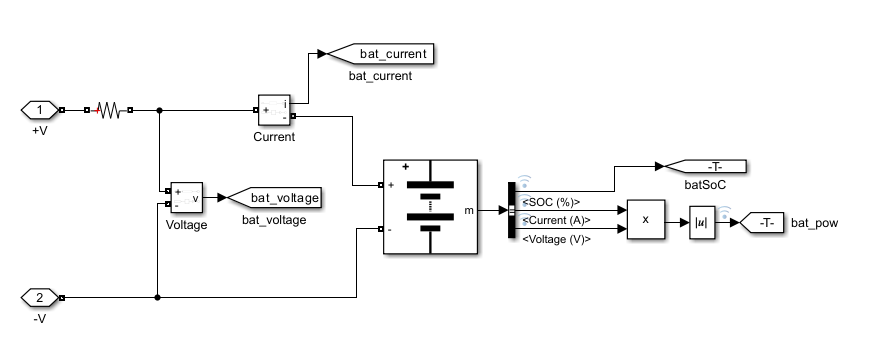
\includegraphics[totalheight=5cm]{Figures/bess.png}
	\caption{Battery Storage System}
	%	\label{fig:verticalcell}
\end{figure}

\subsection{Load Profile}
Internally, most of the appliances operate on DC \cite{42}. With the improvement in technology such as USB power delivery (USB-PD) standards, appliances such as LCD TV, laptops and monitors can be powered directly from USB connection.  The load profile provided in figures 4.3 – 4.7 are utilised to model various load conditions experienced by the units over a 24-hour period.
\begin{figure}[H]
	\centering
	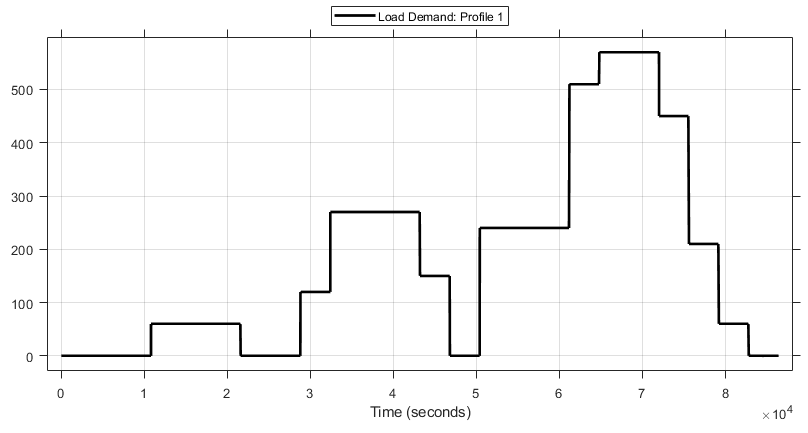
\includegraphics[totalheight=8cm]{Figures/ldp1.png}
	\caption{Load demand: Profile 1}
	%	\label{fig:verticalcell}
\end{figure}
\begin{figure}[H]
	\centering
	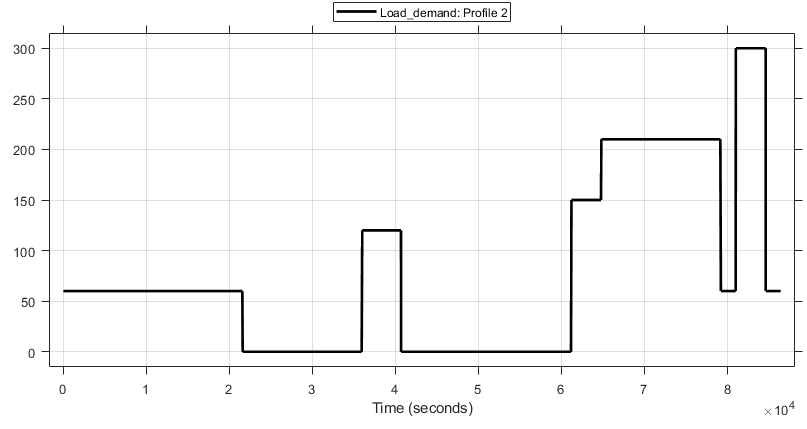
\includegraphics[totalheight=8cm]{Figures/ldp2.png}
	\caption{Load demand: Profile 2}
	%	\label{fig:verticalcell}
\end{figure}
\begin{figure}[H]
	\centering
	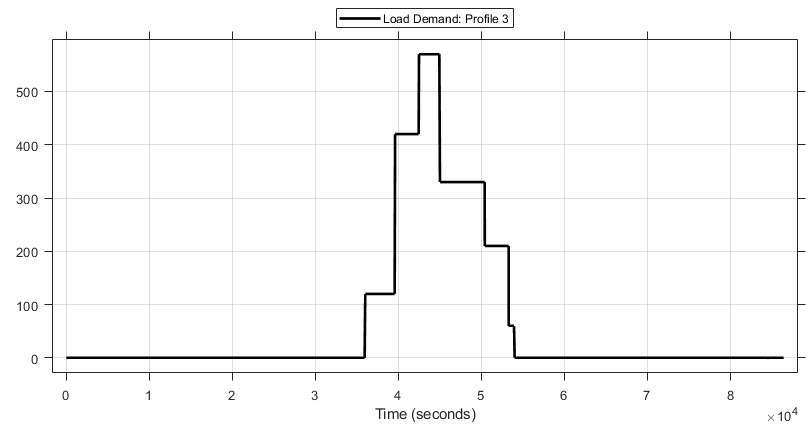
\includegraphics[totalheight=8cm]{Figures/ldp3.png}
	\caption{Load demand: Profile 3}
	%	\label{fig:verticalcell}
\end{figure}
\begin{figure}[H]
	\centering
	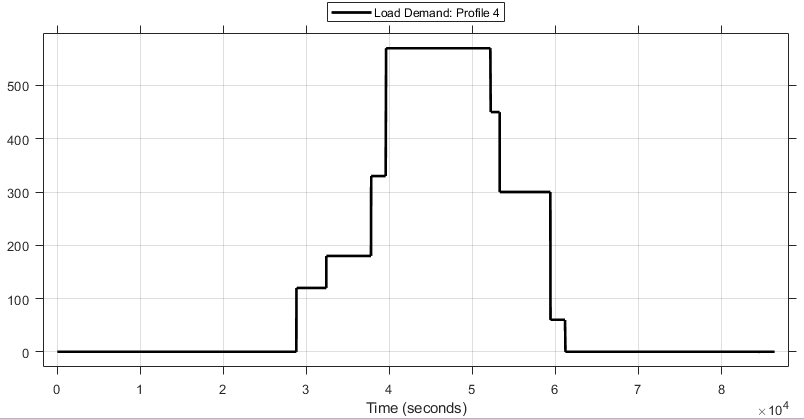
\includegraphics[totalheight=8cm]{Figures/ldp4.png}
	\caption{Load demand: Profile 4}
	%	\label{fig:verticalcell}
\end{figure}
Matlab Signal editor block is used to produce load profiles during simulation time.
\begin{figure}[H]
	\centering
	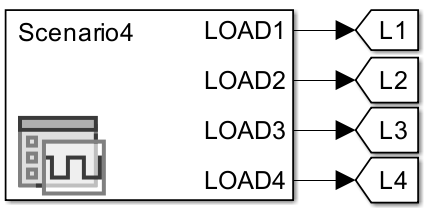
\includegraphics[totalheight=4cm]{Figures/load profile selector.png}
	\caption{Load profile waveform selector}
	%	\label{fig:verticalcell}
\end{figure}
\begin{figure}[H]
	\centering
	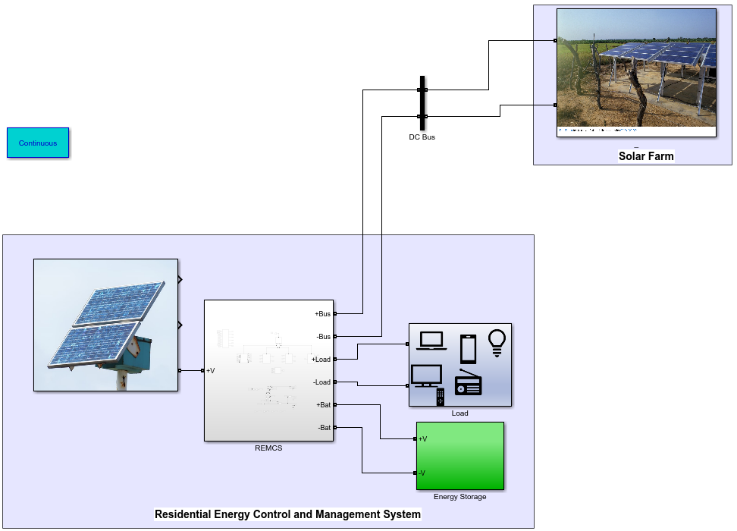
\includegraphics[totalheight=10cm]{Figures/REMCS.png}
	\caption{REMCS unit Matlab overview}
	%	\label{fig:verticalcell}
\end{figure}

Figure 4.9 displayed above illustrates a Matlab/Simulink representation of an REMCS unit connected to a solar farm through a DC MG. Units’ configuration can be modified by addition and or removal of ESS and BSS. In the REMCS block, an MPPT system interfaces with the PV module, and a bidirectional DC-DC converter connects to the external Grid. Several switches are employed to control the grid. The load block consists of four distinct resistive loads that are turned at different interval to produce the load profiles discussed.\par

\begin{figure}[H]
	\centering
	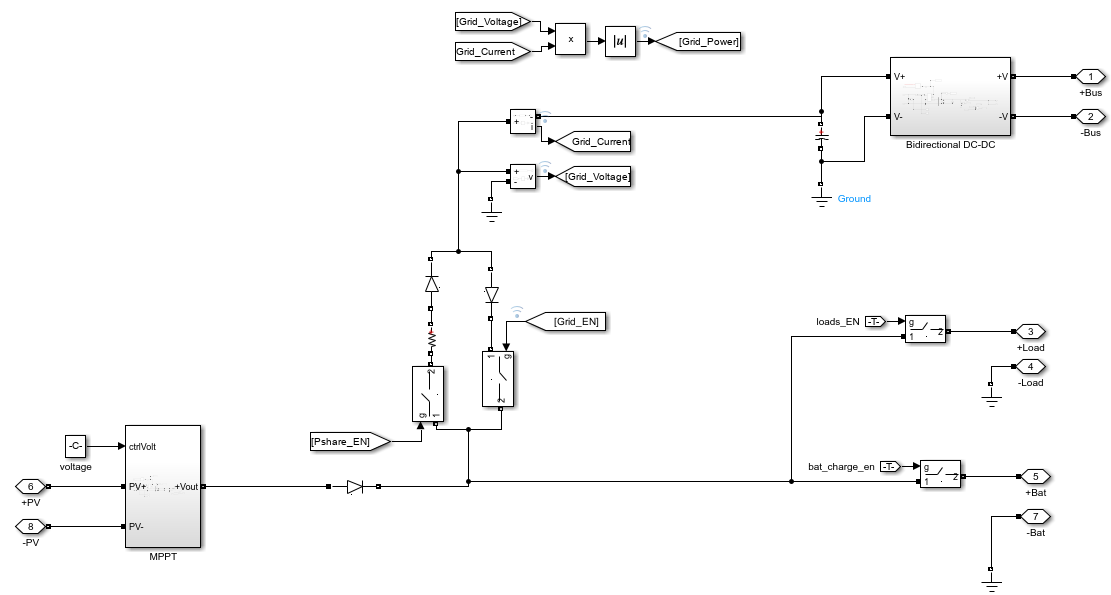
\includegraphics[totalheight=6cm]{Figures/remcs nano grid.png}
	\caption{REMCS nano grid}
	%	\label{fig:verticalcell}
\end{figure}
The load block consists of four distinct resistive loads that are turned at different interval to produce the load profiles discussed.\par
\begin{figure}[H]
	\centering
	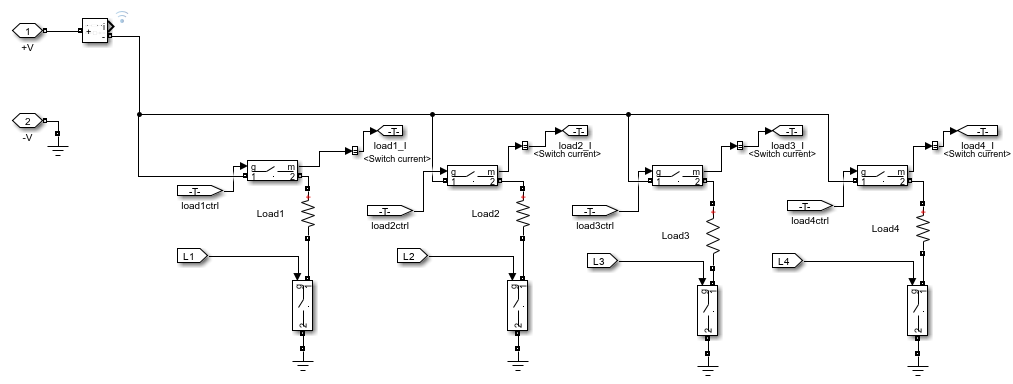
\includegraphics[totalheight=6cm]{Figures/loads control circuit.png}
	\caption{Loads control circuit}
	%	\label{fig:verticalcell}
\end{figure}
The load demand for the load profiles is determined by adding up the total power consumption of all activated loads as depicted in the figure below.\par
\begin{figure}[H]
	\centering
	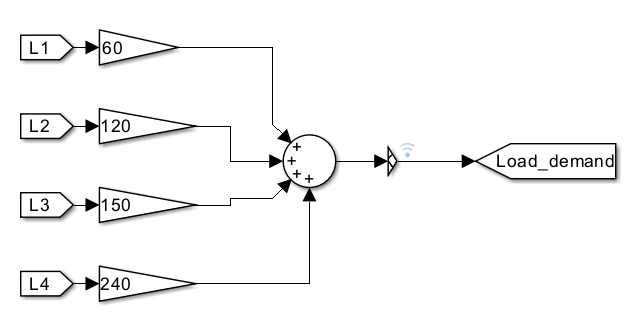
\includegraphics[totalheight=6cm]{Figures/load demand block.png}
	\caption{Load demand block}
	%	\label{fig:verticalcell}
\end{figure}
\section{REMCS Design Logic }
\subsection{State Observer}
The Systems of Systems framework allows REMCS units operate fully independent without direct communication to other units in the grid. The state observer REMCS, using power flow and voltage measurements can determine the state of the grid and respond accordingly.\par
The Systems of Systems philosophy empowers REMCS units to operate as self-contained entities, operating independently without the necessity for direct communication with other units interconnected in the grid. Instead of relying on constant coordination or centralized control, these REMCS units are designed to function autonomously, ensuring flexibility and robustness in the overall system.\par
Within this framework, a state observer is integrated into the REMCS. This observer uses power flow and voltage measurements to assess and monitor the state of the grid. By continuously analysing these key parameters, the state observer can determine the health, performance, and stability of the grid at any given moment.\par
This capability provides several advantages. First, it enables each REMCS unit to make informed decisions in real-time, optimizing its own operations based on the grid's condition. Second, it enhances the grid's resilience since REMCS units can respond to changes or disturbances independently.\par
\begin{figure}[H]
	\centering
	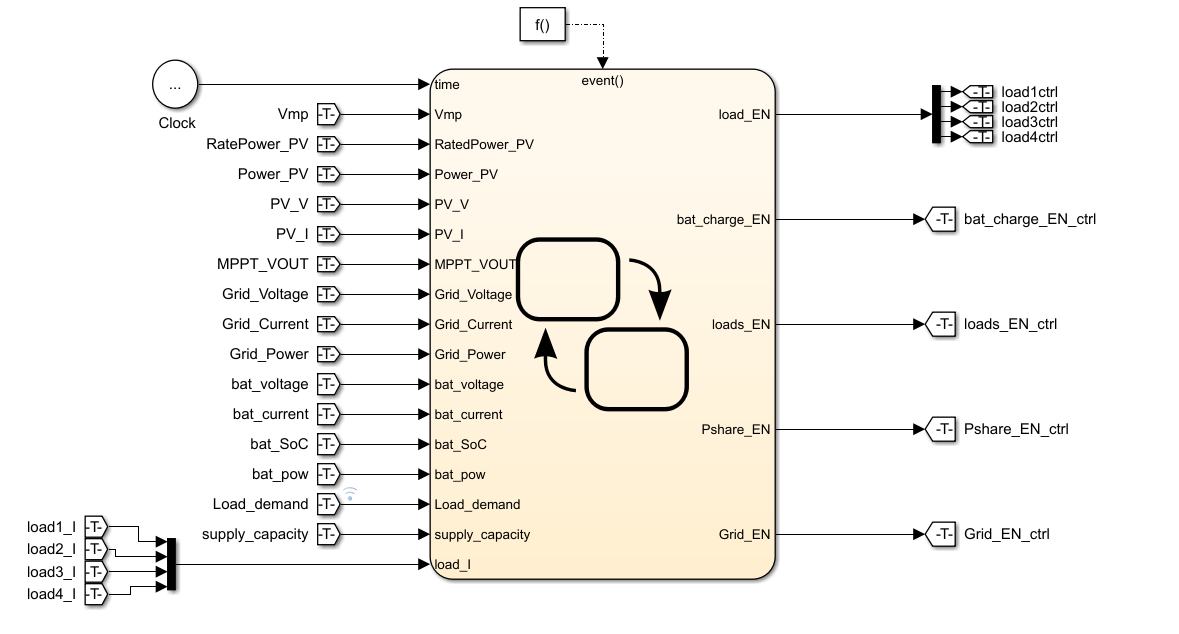
\includegraphics[totalheight=8cm]{Figures/statechart block.png}
	\caption{State chart block}
	%	\label{fig:verticalcell}
\end{figure}
The state chart block transitions the REMCS unit to four distinct states whereby each resource configures the system resource for optimal performance. These states represent different operational modes that the REMCS unit can adapt to as it interacts with the grid. Each state is designed to align with specific objectives and requirements, optimising resource allocation and utilisation. Three states are connected to Start, Running on Battery, PowerShare and charging.\par
\subsubsection{Running on Battery State}
The criteria for transitioning into the Running on Battery state depend on two key factors: the availability of solar power and whether the PV modules have achieved their maximum power point voltage (Vmp). The substates implement load shedding when the battery SoC goes below 30\% by reducing supply capacity. The systems leave this state when bat\_SoC goes above the last recorded SoC before going into Running on Battery mode.\par
\begin{figure}[H]
	\centering
	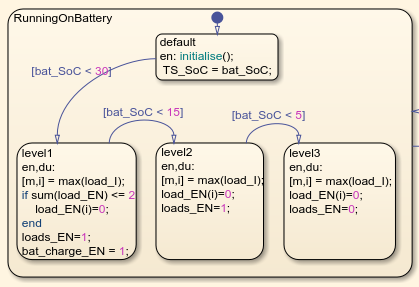
\includegraphics[totalheight=8cm]{Figures/running on battery.png}
	\caption{Running on battery}
	%	\label{fig:verticalcell}
\end{figure}
\subsubsection{Charging State}
The system transitions into a "Charging" state whenever the State of Charge (SoC) drops below 100\%. Upon entering this state, default configurations are applied. Within the Charging state, there are two priority charge substates, PR\_CHRG\_LVL2 and PR\_CHRG\_LVL3, designed to prioritise battery charging then load servicing.
During the PR\_CHRG\_LVL2 substate, load reduction measures are activated when the battery's SoC is below 50\%. Charging continues until the SoC exceeds 75\%, at which point load reduction is lifted.

\subsubsection{Power Share State}
Upon reaching a battery State of Charge of 100\%, and when the photovoltaic (PV) module generates an excess of energy beyond the local load requirements, the system enters a "Power-Share" state. In this state, the system is perceived as an energy source by both the central controller and any other units connected to this system.\par
\begin{figure}[H]
	\centering
	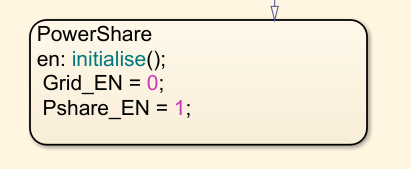
\includegraphics[totalheight=4cm]{Figures/power share state.png}
	\caption{Power Sharing}
	%	\label{fig:verticalcell}
\end{figure}
\section{Model parameters}
The performance of the EMS is determined by the following:\par
Bat\_SoC – The energy storage system plays a crucial role in enhancing grid reliability by supplying power during periods when energy sources may not be dependable. It is imperative to prioritize battery charging whenever Renewable Energy Sources (RES) are actively generating power.\par
SF\_SoC (Solar farm state of charge)– The energy storage system within the solar farm provides power to all REMCS units and plays an important role in maintaining grid voltage stability. When systems operate autonomously, it is essential that they refrain from drawing power as the State of Charge (SoC) of the solar farm's energy storage system approaches depletion.\par
Loads – Predicting and planning for load demand presents a challenge, primarily because consumers do not adhere to a rigid schedule for switching on their loads. In microgrid systems, demand-side management strategies, as discussed in \cite{43}, have been adopted to enhance efficiency, reduce utility bills, and serve various other objectives.\par
In summary, the integration of an EMS into the grid is anticipated to enhance the charging rate of local Battery Energy Storage Systems (BESS), particularly during daylight hours when PV modules generate power. This integration also plays a vital role in maintaining grid stability by reducing the discharge rate of BESS. Additionally, the Energy Management System (EMS) is responsible for effectively directing surplus power generated by PV modules back into the grid. To achieve these objectives, the EMS can implement strategies to reduce overall load demand.\par
The benchmarks mentioned above will undergo testing within all four scenarios, with each load profile depicted in figures 4.3 through 4.7 being applied. This testing procedure will serve as the means to assess the performance of the EMS.
	\begin{table}[!ht]
	\begin{center}
		\caption{Scenario 1: Model setup parameters}
		%\label{tab:table2}
		\begin{tabular}{|p{6cm}|p{8cm}|} % <-- Alignments: 1st column left, 2nd middle and 3rd right, with vertical lines in between
			\hline
			\textbf{Irradiance profile } & \textbf{Figure 4.1}\\
			\hline
			Battery size and capacity	& Nominal voltage: 48 V DC \\
										& Capacity: 22Ah\\
					  					& Initial SOC: 50\% \\
					  					\hline
			Load Size 					& Minimum: 60(W)\\
					 					& Maximum: 570(W)\\
										\hline
			PV module		 			& Maximum power: 240.53(W)\\
										& Vmp: 30.72(V)\\
										& Imp: 7.83(A)\\
										\hline
			Load profiles used & Case study 1: Load profile 1(Figure 4.3)\\
			\hline
			Load profiles used & Case study 4: Load profile 1(Figure 4.7)\\
			\hline
		\end{tabular}
	\end{center}
\end{table}
\subsection{Case study 1}
\begin{figure}[H]
	\centering
	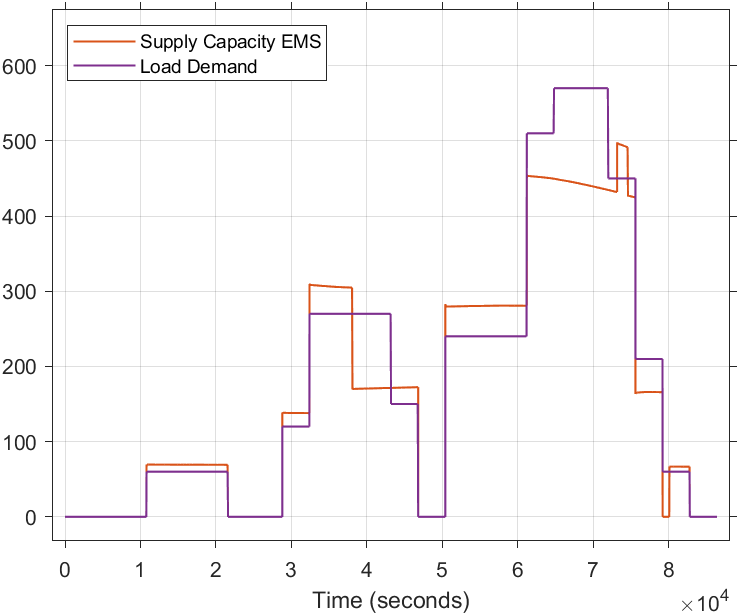
\includegraphics[totalheight=8cm]{Figures/supply capacity with ems v load demand.png}
	\caption{Supply capacity with EMS v load demand}
	%	\label{fig:verticalcell}
\end{figure}
\begin{figure}[H]
	\centering
	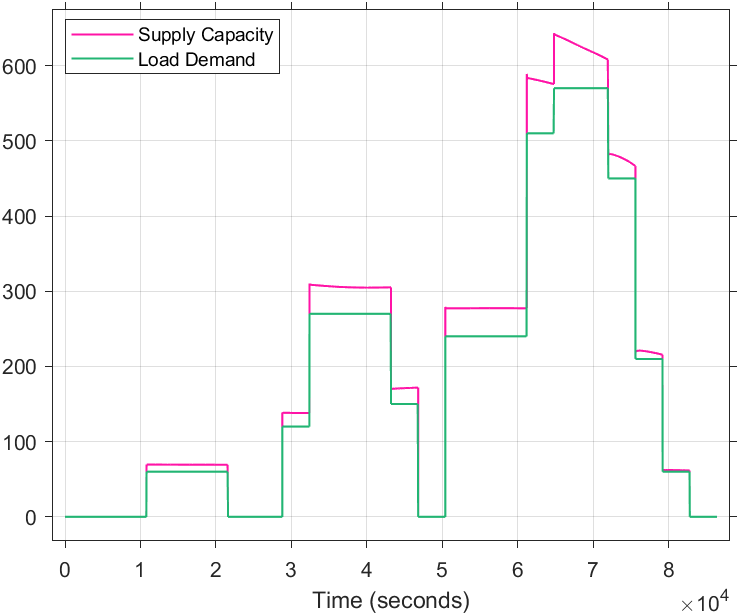
\includegraphics[totalheight=8cm]{Figures/supply capacity with non-ems v load demand.png}
	\caption{non-EMS Supply capacity with v load demand}
	%	\label{fig:verticalcell}
\end{figure}
To satisfy the load demand, the supply capacity must consistently equal or exceed the load demand. The results obtained in figure 4.17 demonstrate the capability of the energy source within the DC MG to fulfil the unit's energy load profile, particularly in the non-EMS integrated scenarios. \par
The inability of the EMS-Integrated DC MG to meet load demand can be traced to its energy prioritization feature, which allocates a portion of the available energy for battery charging.\par
Consequently, this feature results in a noticeable 10\% improvement in the state of charge (SoC) of local storage when compared to the non-EMS system, as illustrated in Figure 4.18 at time ${5\times10^4 s}$.
\begin{figure}[H]
	\centering
	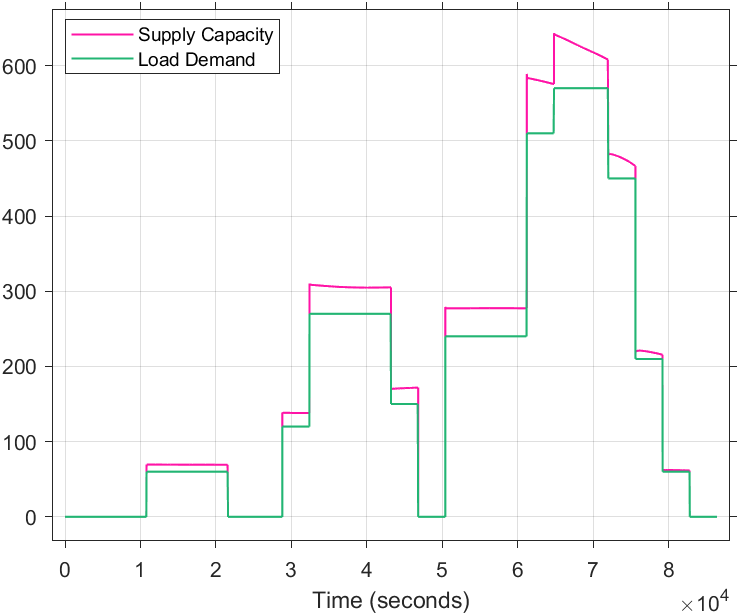
\includegraphics[totalheight=8cm]{Figures/supply capacity with non-ems v load demand.png}
	\caption{Local Storage SoC EMS v non-EMS system}
	%	\label{fig:verticalcell}
\end{figure}
The initial differences in SoC observed after ${3.8\times10^4}$ seconds between the non-EMS DC MG and the EMS-integrated DC MG can be attributed to the EMS's response time when detecting sufficient power from RESs. Peak load demand commences around ${3.8\times10^4}$ seconds, which closely coincides with the moment when PV panels cease power production due to the sunset. During peak demand, the slope remains consistent for both systems, primarily because of the identical load profile and the fact that RES is not generating power. The load demand persists until approximately ${8.4\times10^4}$ seconds, causing a significant decline in the State of Charge (SoC) of both the solar farm and local energy storage. The Solar Farm SoC comparison is shown in figure 4.18  To reduce dependence on external power sources, the EMS restricts the utilization of the solar farm's storage until the local storage drops below 15\% or cannot meet the load demand. Solar farm SoC drops from 50\% at time 0 seconds to 20\% at time 86400. EMS-integrated systems have 16.5\% more storage capacity than the non-EMS system as shown in fig. 4.19
\begin{figure}[H]
	\centering
	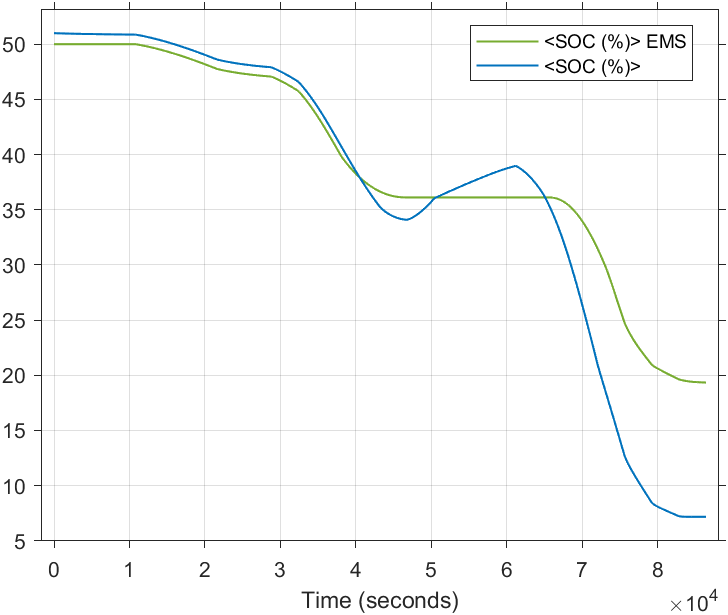
\includegraphics[totalheight=8cm]{Figures/solar farm storage soc ems v non-ems system.png}
	\caption{Solar Farm Storage SoC EMS v non-EMS system}
	%	\label{fig:verticalcell}
\end{figure}
The load demand data for case study 4 is illustrated in figures 4.20 and 4.21, with a specific focus on highlighting the EMS local storage prioritization feature.

\begin{figure}[H]
	\centering
	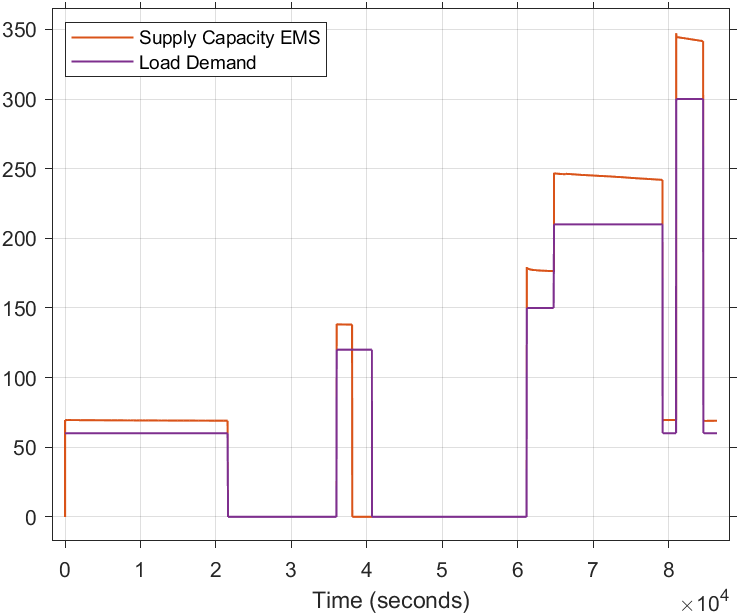
\includegraphics[totalheight=8cm]{Figures/supply capacity ems v load demand.png}
	\caption{Supply capacity EMS v Load demand}
	%	\label{fig:verticalcell}
\end{figure}
\begin{figure}[H]
	\centering
	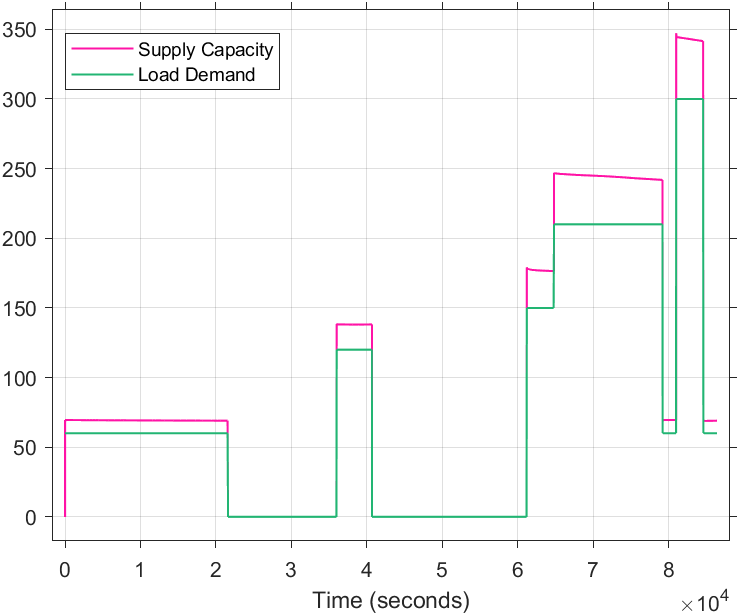
\includegraphics[totalheight=8cm]{Figures/non-ems supply capacity v load demand.png}
	\caption{Non-EMS Supply capacity v Load demand}
	%	\label{fig:verticalcell}
\end{figure}
The comparison of local storage between the EMS and non-EMS systems in Figure 4.21 demonstrates the EMS's early response time and its charging rate. The higher charging rate of EMS systems results from using PV modules exclusively for local battery storage charging, as opposed to non-EMS systems which also have to charge solar farm SoC. \par
Figure 4.20 demonstrates the power sharing feature of the EMS. This feature activates when local storage is charged. Due to its higher charging rate, the EMS can bring the Solar farm SoC within 1\% of the non-EMS system.

\begin{figure}[H]
	\centering
	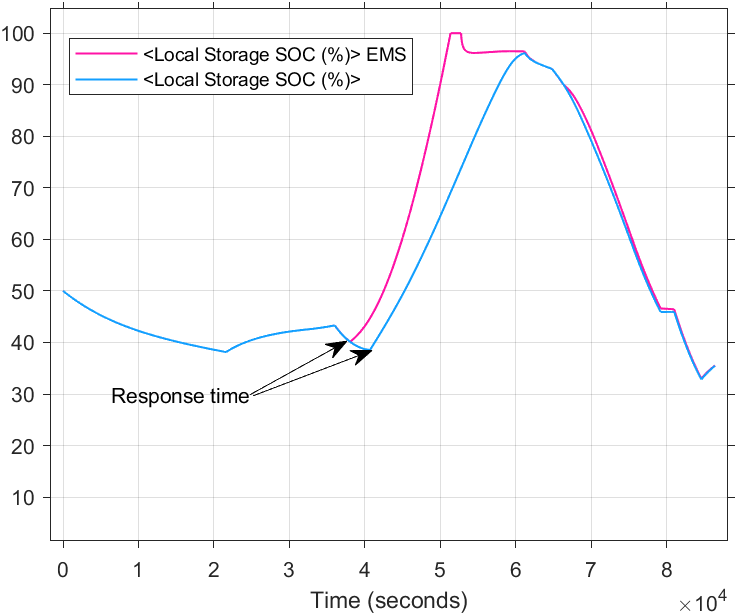
\includegraphics[totalheight=8cm]{Figures/local storage soc ems v non-ems.png}
	\caption{Local Storage SoC EMS v non-EMS}
	%	\label{fig:verticalcell}
\end{figure}
\begin{figure}[H]
	\centering
	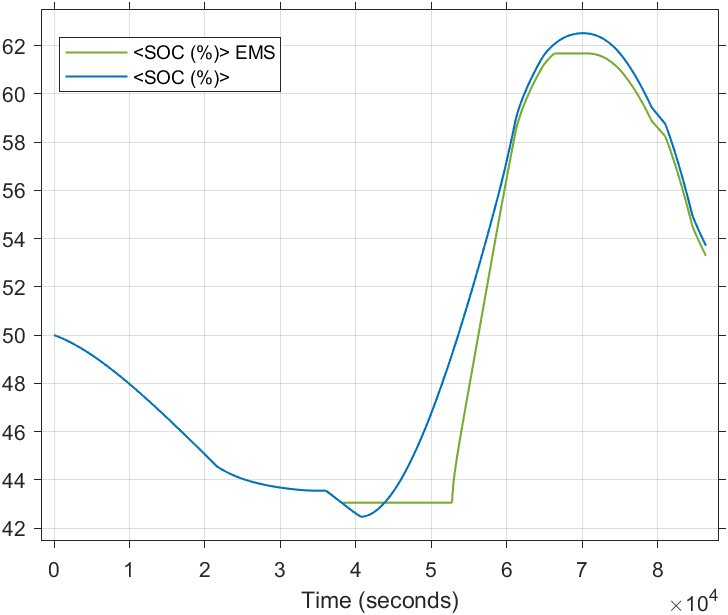
\includegraphics[totalheight=8cm]{Figures/solar farm storage soc ems v non-ems.png}
	\caption{Solar Farm Storage SoC EMS v non-EMS}
	%	\label{fig:verticalcell}
\end{figure}

\subsection{Case Study 2}
	\begin{table}[!ht]
	\begin{center}
		\caption{Scenario 2: Model setup parameters}
		%\label{tab:table2}
		\begin{tabular}{|p{6cm}|p{8cm}|} % <-- Alignments: 1st column left, 2nd middle and 3rd right, with vertical lines in between
			\hline
			\textbf{Irradiance profile } & \textbf{Figure 4.1}\\
			\hline
			Battery size and capacity	& Nominal voltage: 0 V DC \\
			& Capacity: 0Ah\\
			& Initial SOC: 0\% \\
			\hline
			Load Size 					& Minimum: 60(W)\\
			& Maximum: 570(W)\\
			\hline
			PV module		 			& Maximum power: 240.53(W)\\
			& Vmp: 30.72(V)\\
			& Imp: 7.83(A)\\
			\hline
			Load profiles used & Case study 1: Load profile 1(Figure 4.3)\\
			\hline
			Load profiles used & Case study 4: Load profile 1(Figure 4.5)\\
			\hline
		\end{tabular}
	\end{center}
\end{table}
Table 4.4 provides a profile for Unit 2 REMCS, which relies heavily on solar power. In the absence of local energy storage to store excess power generated from the PV modules, the EMS enables the power-sharing module when the load demand is reduced, allowing for efficient use of the surplus energy.

\begin{figure}[H]
	\centering
	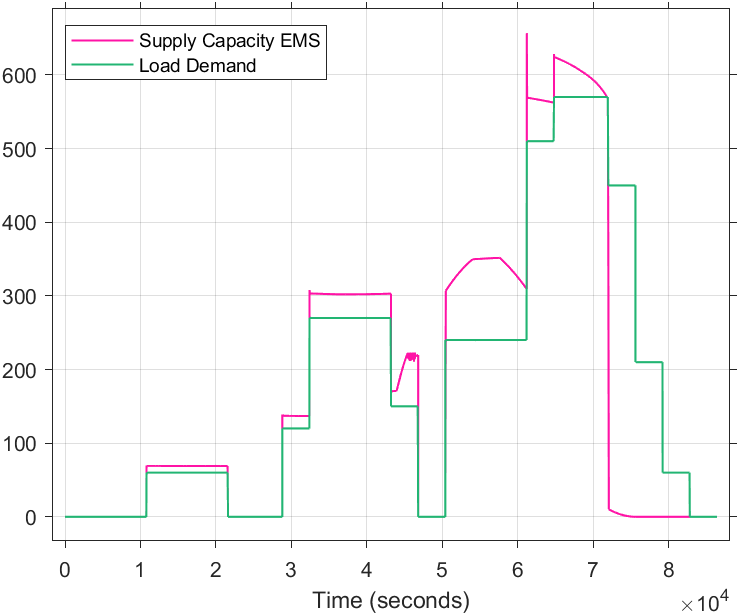
\includegraphics[totalheight=8cm]{Figures/ems supply capacity v load demand.png}
	\caption{EMS Supply capacity v load demand}
	%	\label{fig:verticalcell}
\end{figure}
\begin{figure}[H]
	\centering
	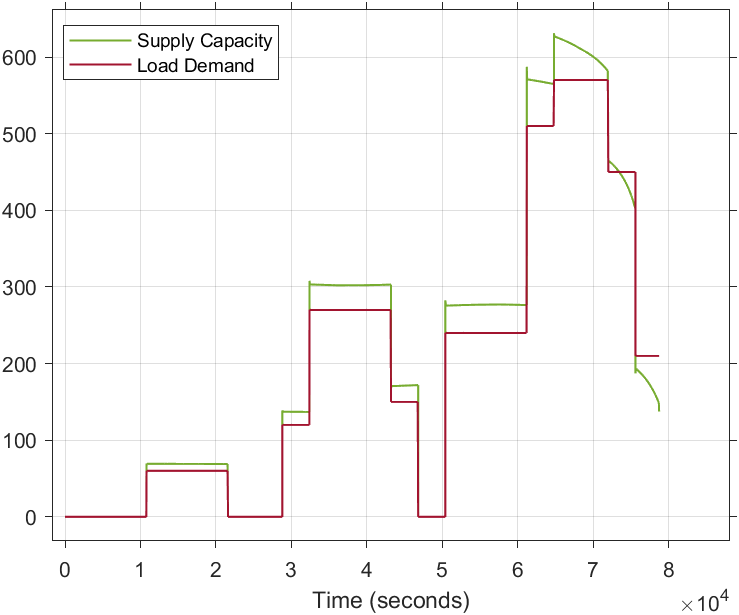
\includegraphics[totalheight=8cm]{Figures/non-ems supply capacity v load demand1.png}
	\caption{Non-EMS Supply capacity v load demand}
	%	\label{fig:verticalcell}
\end{figure}
The load demands versus supply capacity for the two systems are depicted in Figures 4.24 and 4.25. Both systems can meet load demand until ${7.2\times10^4 s}$ seconds for the EMS system and ${7.6\times10^4 s}$seconds for the non-EMS system.

\begin{figure}[H]
	\centering
	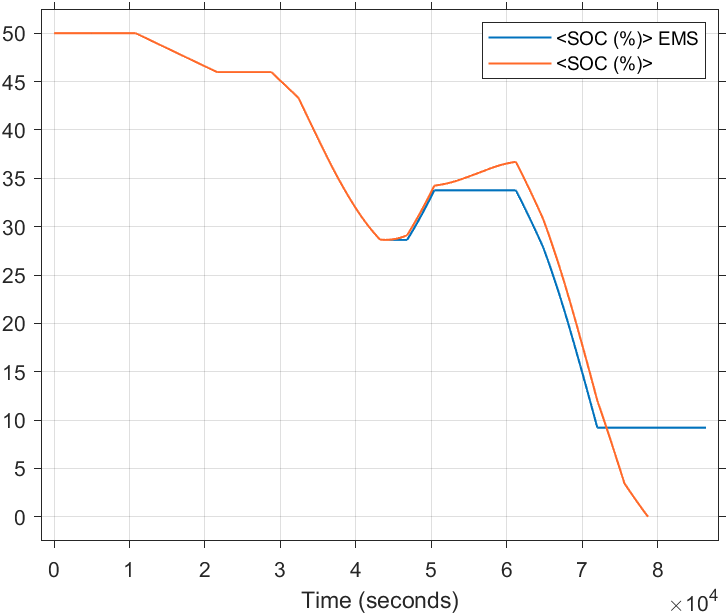
\includegraphics[totalheight=8cm]{Figures/solar farm soc ems v non-ems.png}
	\caption{Solar Farm SoC EMS v non-EMS}
	%	\label{fig:verticalcell}
\end{figure}
Referring to Figure 4.26, the Solar farm gradually decreases its state of charge (SoC) from time 0 seconds to approximately ${4.3\times10^4 s}$seconds. Due to high load demand, the solar farm's SoC increases by 10\% for the EMS system and 15\% for the non-EMS system. The lower SoC in the EMS system compared to the non-EMS system can be attributed to the EMS's prioritisation of local energy storage, which attempts to charge local batteries that are non-existent for this particular unit, this defaults the EMS to Start. Start state is verified in Figure 4.27 from time ${5\times10^4 s}$seconds to time ${6.02\times10^4 s}$seconds.\par

\begin{figure}[H]
	\centering
	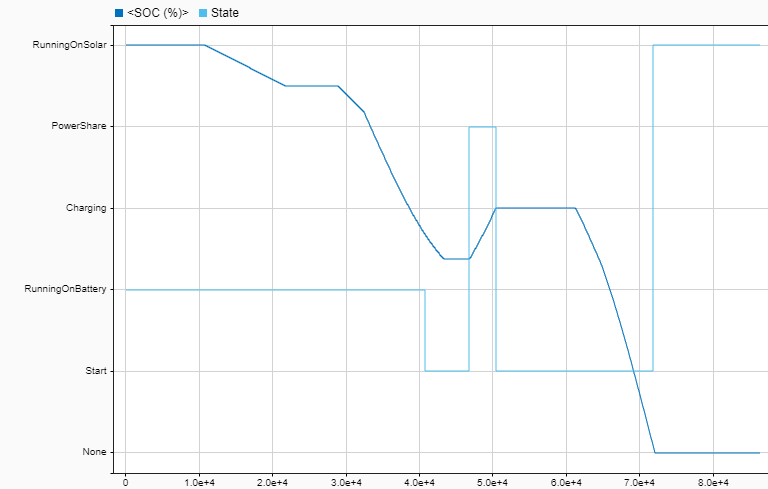
\includegraphics[totalheight=8cm]{Figures/local soc and state transition.png}
	\caption{Local SoC and state transition}
	%	\label{fig:verticalcell}
\end{figure}
\begin{figure}[H]
	\centering
	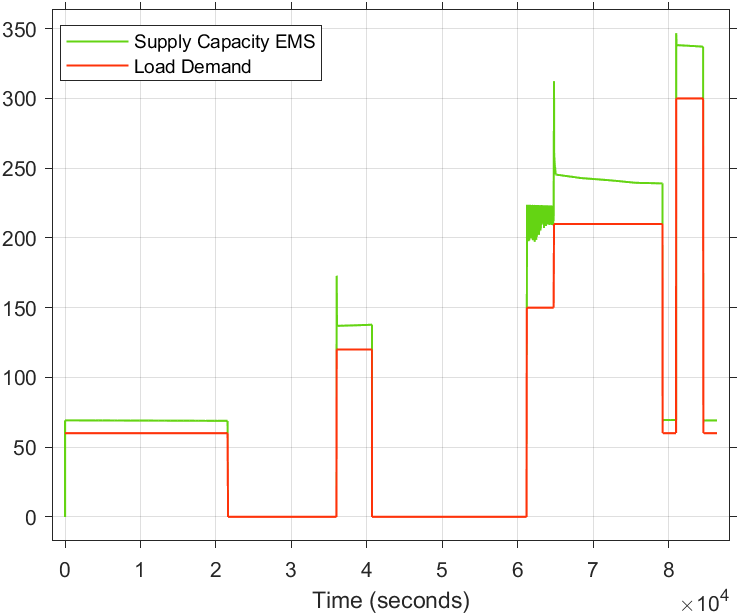
\includegraphics[totalheight=8cm]{Figures/ems supply capacity v load demand1.png}
	\caption{EMS Supply capacity v load demand}
	%	\label{fig:verticalcell}
\end{figure}
\begin{figure}[H]
	\centering
	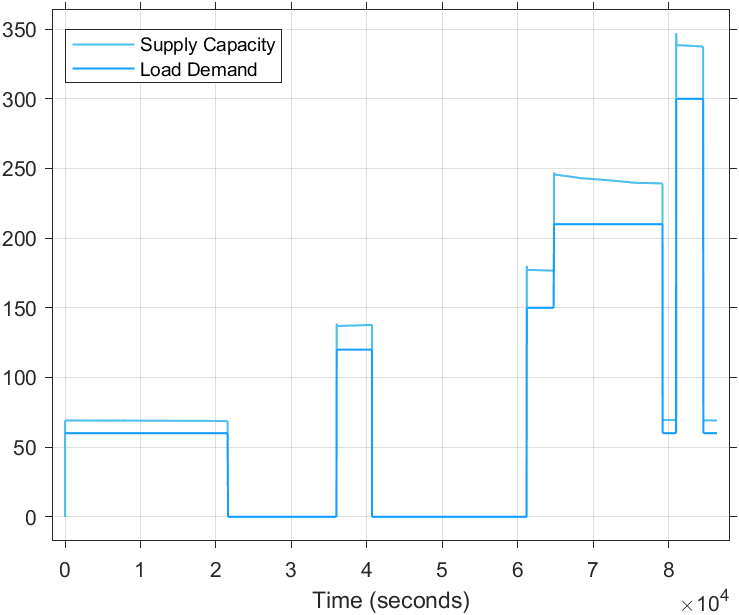
\includegraphics[totalheight=8cm]{Figures/non-ems supply capacity v load demand2.png}
	\caption{Non-EMS Supply capacity v load demand}
	%	\label{fig:verticalcell}
\end{figure}
Supply capacity results for Load Profile 3 are displayed in Figures 4.28 and 4.29. The demand for this profile peaks at 350W, which can be adequately powered by both PV modules and the solar farm source.
Due to this moderate demand, the EMS and non-EMS systems increase the solar farm SoC to 69\% and 71\%, respectively.\par 
In the absence of battery storage detection, the EMS switches to its default Start state, leading to a 2\% lower SoC compared to the non-EMS system as shown in figure 4
\begin{figure}[H]
	\centering
	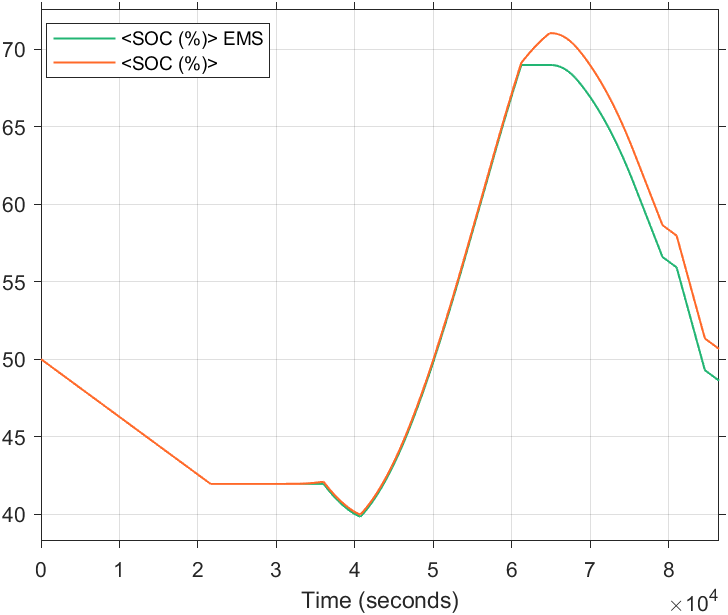
\includegraphics[totalheight=8cm]{Figures/solar farm soc ems v non-ems1.png}
	\caption{EMS supply capacity and state transition}
	%	\label{fig:verticalcell}
\end{figure}

\subsection{Case Study 3}
	\begin{table}[!ht]
	\begin{center}
		\caption{Scenario 3: Model setup parameters}
		%\label{tab:table2}
		\begin{tabular}{|p{6cm}|p{8cm}|} % <-- Alignments: 1st column left, 2nd middle and 3rd right, with vertical lines in between
			\hline
			\textbf{Irradiance profile } & \textbf{Figure 4.1}\\
			\hline
			Battery size and capacity	& Nominal voltage: 0 V DC \\
			& Capacity: 0Ah\\
			& Initial SOC: 0\% \\
			\hline
			Load Size 					& Minimum: 60(W)\\
			& Maximum: 570(W)\\
			\hline
			PV module		 			& Maximum power: 240.53(W)\\
			& Vmp: 30.72(V)\\
			& Imp: 7.83(A)\\
			\hline
			Load profiles used & Case study 1: Load profile 1(Figure 4.3)\\
			\hline
			Load profiles used & Case study 4: Load profile 1(Figure 4.5)\\
			\hline
		\end{tabular}
	\end{center}
\end{table}
Case study 3 presents an REMCS unit which lacks PV module, with no PV panels to charge local batteries, this unit is constantly running on battery.
\begin{figure}[H]
	\centering
	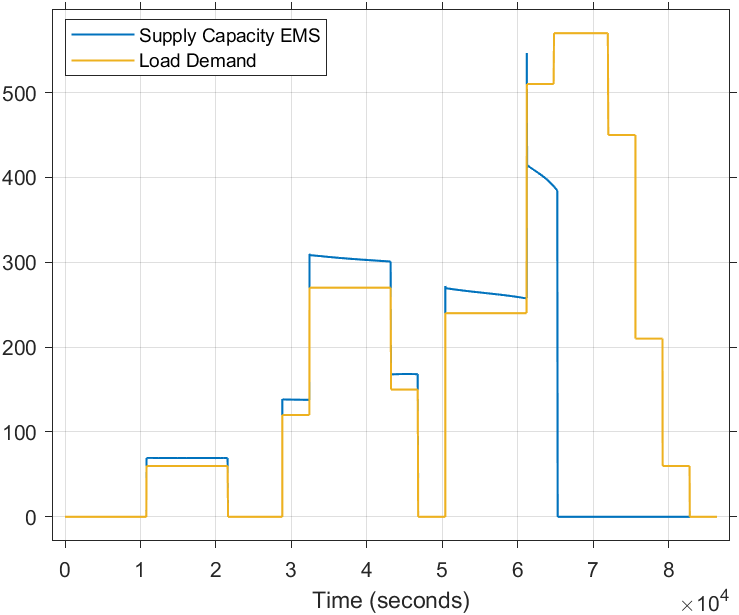
\includegraphics[totalheight=8cm]{Figures/ems supply capacity v load demand2.png}
	\caption{EMS Supply capacity v load demand}
	%	\label{fig:verticalcell}
\end{figure}
\begin{figure}[H]
	\centering
	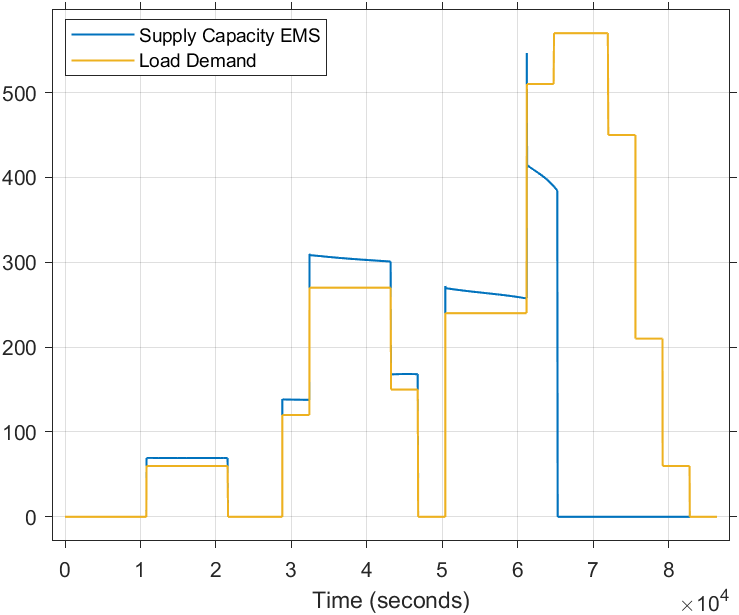
\includegraphics[totalheight=8cm]{Figures/ems supply capacity v load demand2.png}
	\caption{EMS Supply capacity v load demand}
	%	\label{fig:verticalcell}
\end{figure}
\begin{figure}[H]
	\centering
	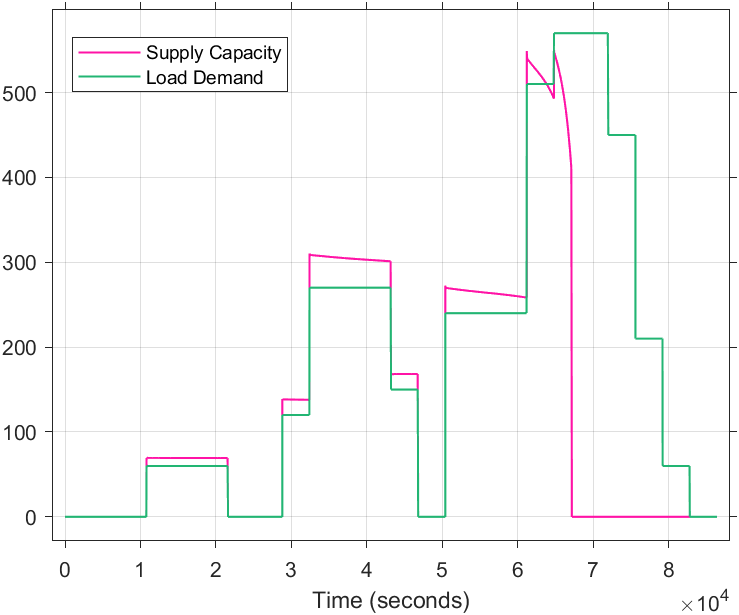
\includegraphics[totalheight=8cm]{Figures/non-ems supply capacity v load demand3.png}
	\caption{Non-EMS Supply capacity v load demand}
	%	\label{fig:verticalcell}
\end{figure}

When comparing load demand and supply capacity between figures 4.32 and 4.33, it is evident that EMS and non-EMS systems generally exhibit similar responses. However, there is a noticeable deviation occurring between ${6.10\times10^4 s}$seconds and ${7\times10^4 s}$seconds. During this time frame, the REMCS reduces supply capacity 1863 seconds earlier compared to the non-EMS system.\par

The early drop of supply capacity in the EMS system is directly attributable to EMS energy saving feature which cuts off all loads when SoC drops below 10\%, as it can be show in Figure 4.34.\par

\begin{figure}[H]
	\centering
	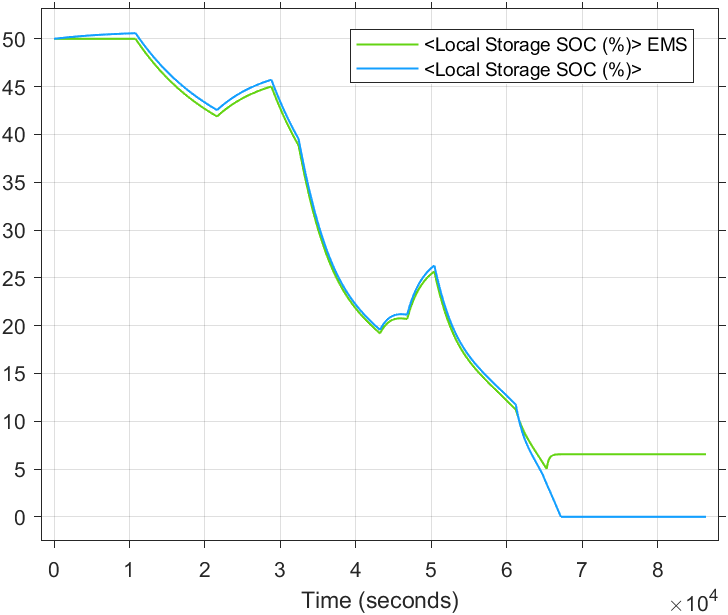
\includegraphics[totalheight=8cm]{Figures/local storage soc ems v non-ems1.png}
	\caption{Local storage SoC EMS v non-EMS}
	%	\label{fig:verticalcell}
\end{figure}
Load profile 4 demonstrates the load shedding feature of the EMS which reduces supply capacity to extend battery usage.\par
\begin{figure}[H]
	\centering
	\includegraphics[totalheight=8cm]{Figures/EMS Supply capacity v load demand3.png}
	\caption{EMS Supply capacity v load demand}
	%	\label{fig:verticalcell}
\end{figure}
\begin{figure}[H]
	\centering
	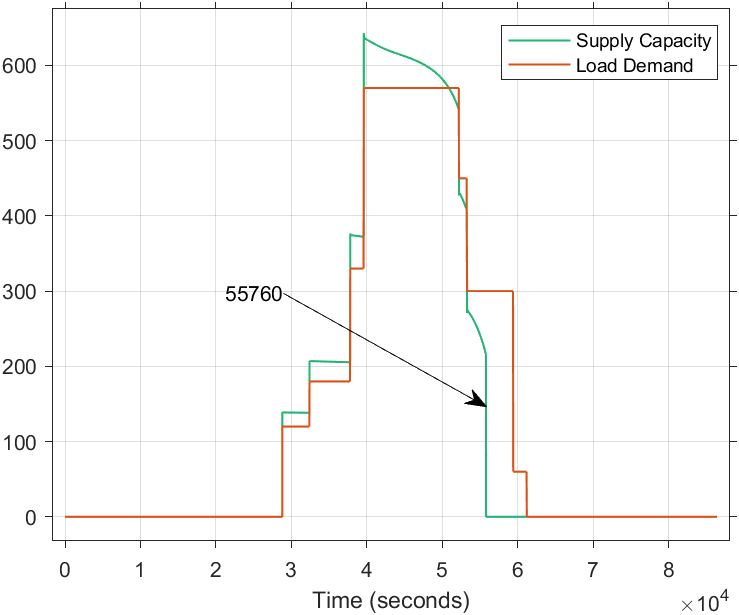
\includegraphics[totalheight=8cm]{Figures/non-ems supply capacity v load demand4.png}
	\caption{Non-EMS Supply capacity v load demand}
	%	\label{fig:verticalcell}
\end{figure}
The time differences between the systems are shown in figure 4.37 and 4.38. As a result of load shedding, EMS gains a 2140 seconds before dropping supply to zero.
\begin{figure}[H]
	\centering
	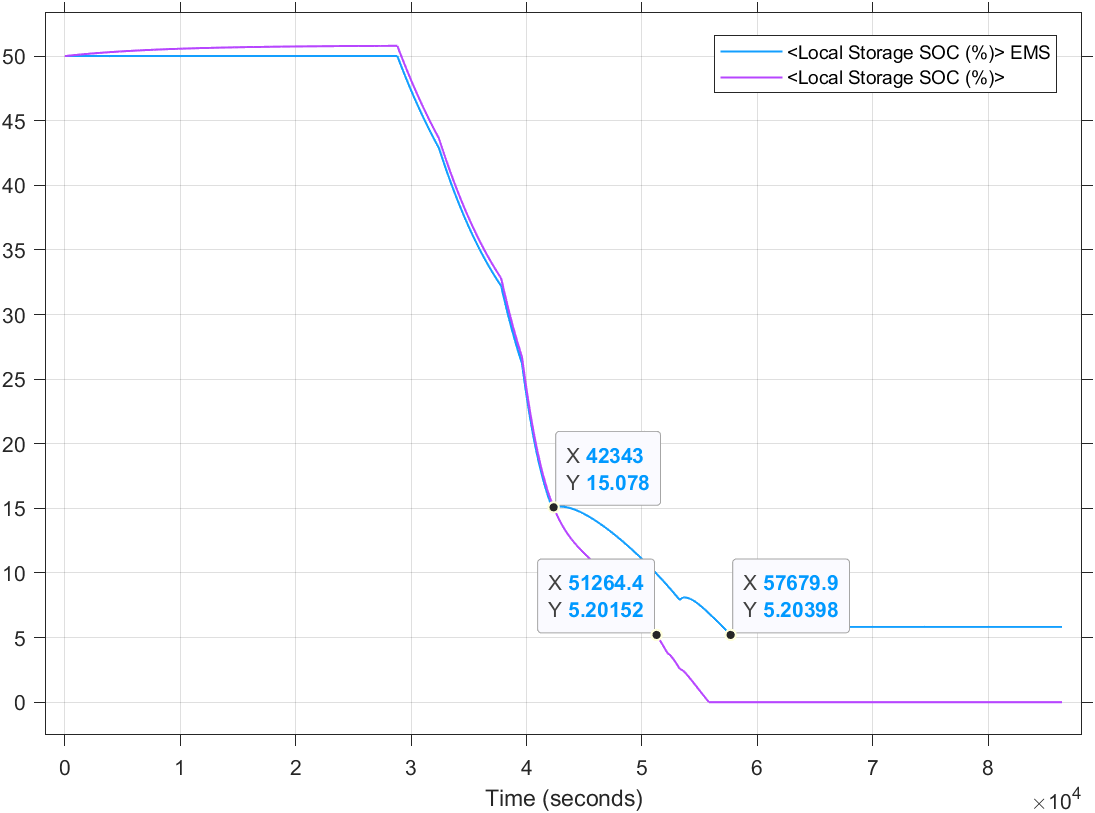
\includegraphics[totalheight=8cm]{Figures/local storage soc ems v non-ems2.png}
	\caption{Local storage SoC EMS v non-EMS}
	%	\label{fig:verticalcell}
\end{figure}
\begin{figure}[H]
	\centering
	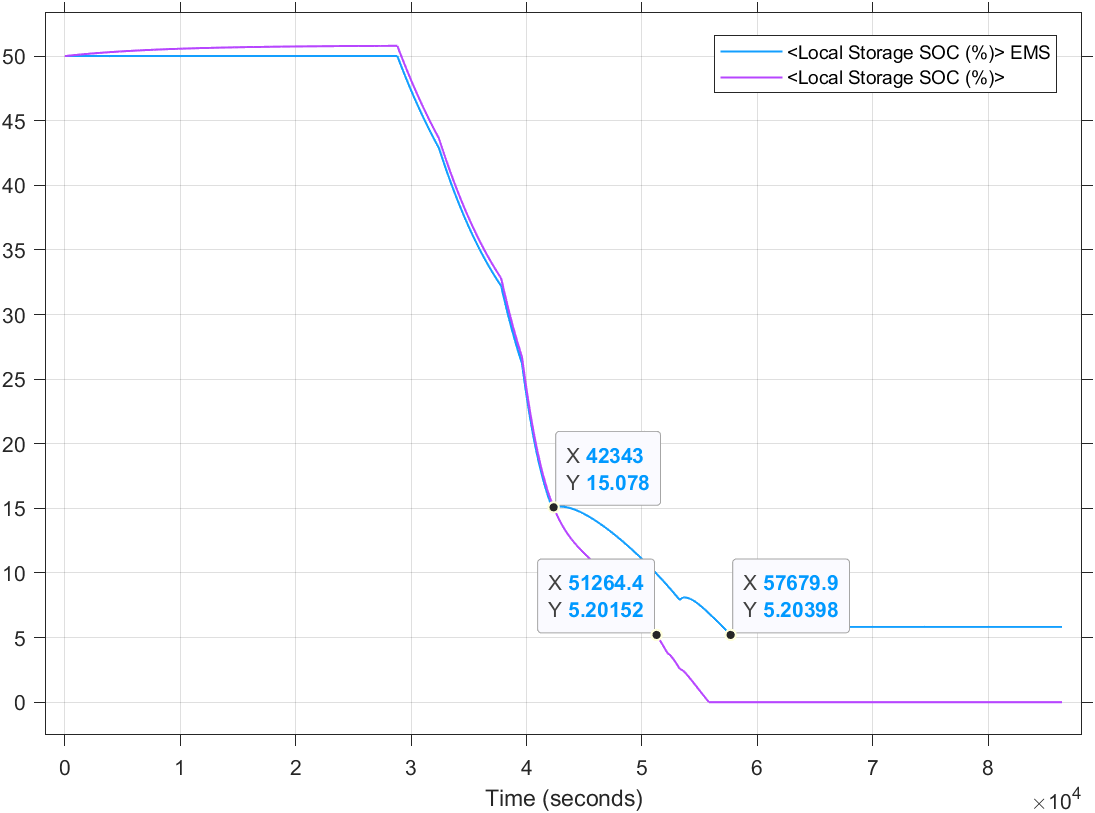
\includegraphics[totalheight=8cm]{Figures/local storage soc ems v non-ems2.png}
	\caption{Local storage SoC EMS v non-EMS}
	%	\label{fig:verticalcell}
\end{figure}
\begin{figure}[H]
	\centering
	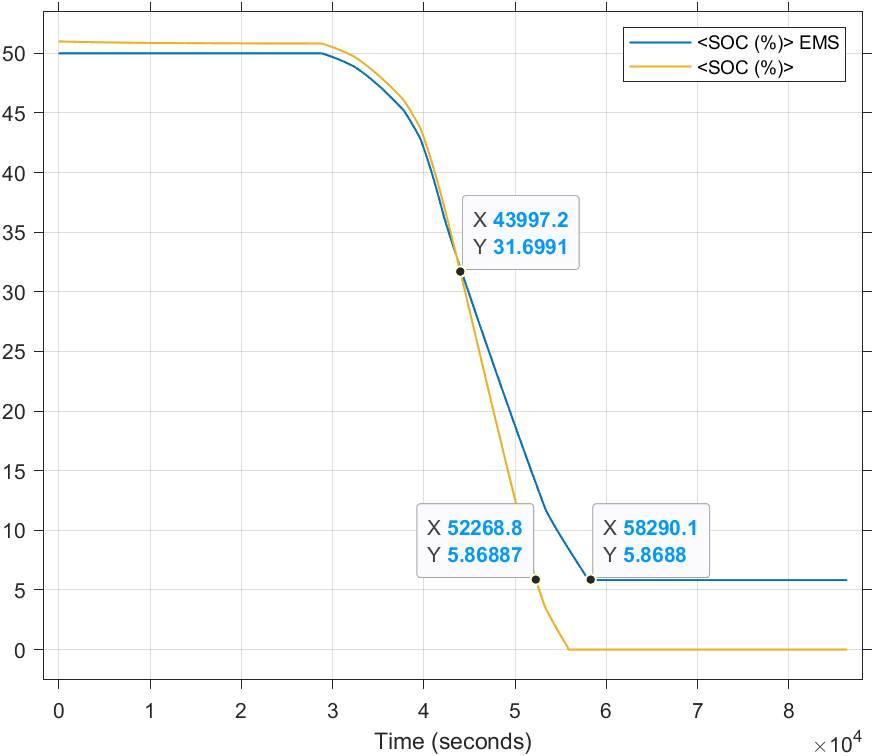
\includegraphics[totalheight=8cm]{Figures/solar farm soc ems v non-ems2.png}
	\caption{Solar Farm SoC EMS v non-EMS}
	%	\label{fig:verticalcell}
\end{figure}
The results of the improvement in the Energy Management System due to the implementation of load shedding are shown in Figures 4.38 and 4.39. The rate of discharge of SoC, or discharge rate, for the local energy storage has been reduced to -2.30\% per hour, compared to -3.96\% per hour in the non-EMS system. Similarly, for the solar farm, the discharge rate has been reduced to -6.5\% per hour, compared to 11\% per hour in the non-EMS system.

\subsection{Case Study 4}
\begin{table}[!ht]
	\begin{center}
		\caption{Scenario 3: Model setup parameters}
		%\label{tab:table2}
		\begin{tabular}{|p{6cm}|p{8cm}|} % <-- Alignments: 1st column left, 2nd middle and 3rd right, with vertical lines in between
			\hline
			\textbf{Irradiance profile } & \textbf{Figure 4.1}\\
			\hline
			Battery size and capacity	& Nominal voltage: 0 V DC \\
			& Capacity: 0Ah\\
			& Initial SOC: 0\% \\
			\hline
			Load Size 					& Minimum: 60(W)\\
			& Maximum: 570(W)\\
			\hline
			PV module		 			& Maximum power: 0(W)\\
			& Vmp: 0(V)\\
			& Imp: 0(A)\\
			\hline
			Load profiles used & Case study 1: Load profile 1(Figure 4.3)\\
				 			   & Case study 2: Load profile 1(Figure 4.4)\\
				 			   & Case study 3: Load profile 1(Figure 4.5)\\
				 			   & Case study 4: Load profile 1(Figure 4.6)\\
			\hline
		\end{tabular}
	\end{center}
\end{table}

Case study 4 presents a unit which has no energy storage system or PV panel. It is an entirely grid-dependent unit which relies on solar farm and excess power from other units. The supply capacity response for this configuration is shown in figures 4.8.24 and 4.8.25. The EMS has control measures to prevent total grid collapse by completely disabling loads, figure 37 shows supply capacity being dropped to zero. The discontinuity on the non-EMS system in figure 38 is a result of Matlab simulation being unable to simulate a grid collapse condition due to hardware limitations.

\begin{figure}[H]
	\centering
	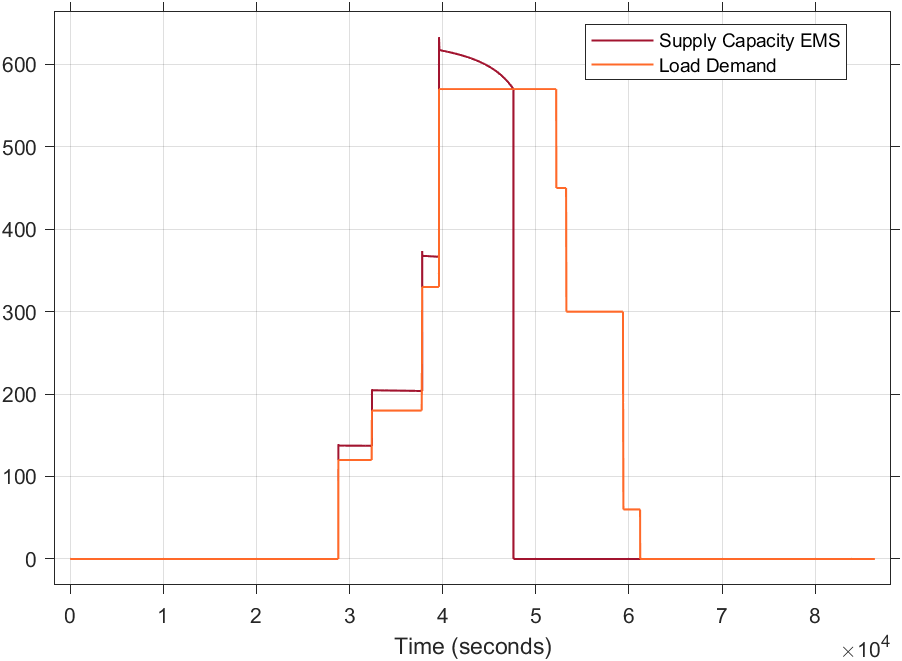
\includegraphics[totalheight=8cm]{Figures/ems supply capacity v load demand4.png}
	\caption{EMS Supply capacity v load demand}
	%	\label{fig:verticalcell}
\end{figure}
\begin{figure}[H]
	\centering
	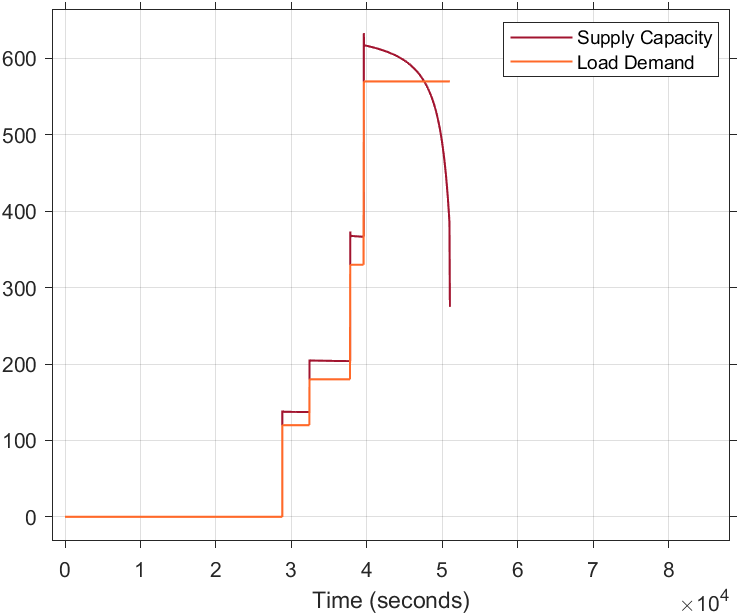
\includegraphics[totalheight=8cm]{Figures/non-ems supply capacity v load demand5.png}
	\caption{non-EMS Supply capacity v load demand}
	%	\label{fig:verticalcell}
\end{figure}
\section{Lab-Developed Working System Setup}
A functional system was developed in the lab, as depicted in Figure 4.9.1. Solar panels are mounted outside. The computers use Matlab Simulink to receive external data, process it, and display the system's real-time operation, The DC loads consist of car headlamps with power ratings between 60W and 120W. These lamps are connected in various combinations to simulate household loads, including cell phone charging stations. Additionally, one of the units uses a DC fridge as a load.

\begin{figure}[H]
	\centering
	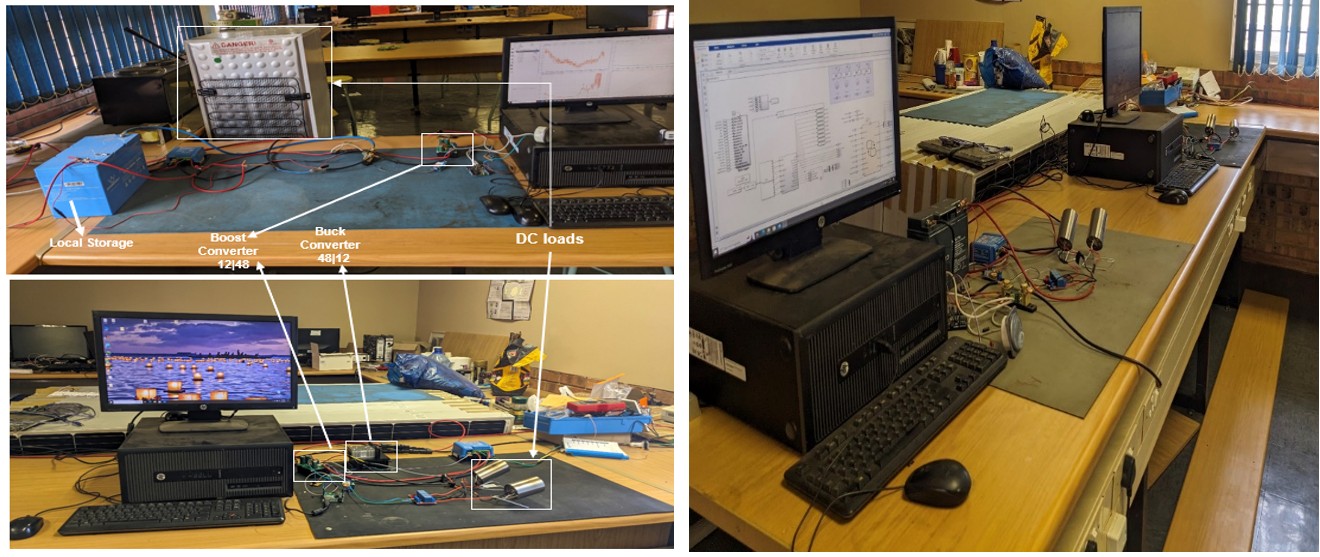
\includegraphics[totalheight=6cm]{Figures/Lab setup of four units DC microgrid.png}
	\caption{Lab setup of four units DC microgrid}
	%	\label{fig:verticalcell}
\end{figure} 
The data obtained from the models was collected for a period of 5 days in which some loads were switched at random intervals to simulate everyday appliances usages. The purpose of this data collection was to analyse the behaviour of electrical loads in a typical household setting. By randomly switching loads, the object was to create a realistic representation of appliance usage patterns, including peak usage times and energy consumption fluctuations. This approach allows for a more accurate assessment of the models' performance in managing energy demand.
\begin{table}[!ht]
	\begin{center}
		\caption{Scenario 3: Model setup parameters}
		%\label{tab:table2}
		\begin{tabular}{|p{6cm}|p{8cm}|} % <-- Alignments: 1st column left, 2nd middle and 3rd right, with vertical lines in between
			\hline
			Battery size and capacity	& Nominal voltage: 12V DC \\
			& Capacity: 100Ah\\
			\hline
			Load Size 					& Minimum: 60(W)\\
			& Maximum: 570(W)\\
			\hline
			PV module		 			& Maximum power: 330(W)\\
			& Vmp: 36.92(V)\\
			& Imp: 8.14(A)\\
			\hline
		\end{tabular}
	\end{center}
\end{table}
The five-day supply capacity v load demand shown in figure 4.9.2 indicates a well-managed load demand, power saving mode is enabled whenever demand exceeds supply.

\begin{figure}[H]
	\centering
	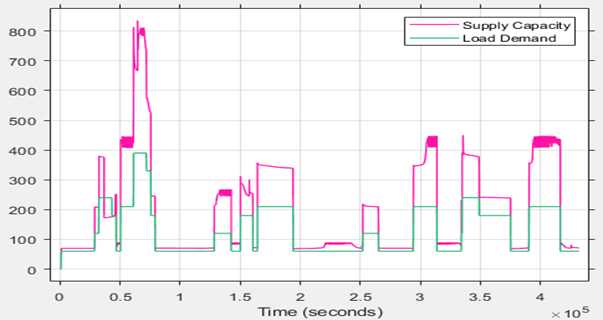
\includegraphics[totalheight=8cm]{Figures/Unit 1 5-day Supply v Load Demand.png}
	\caption{Unit 1 5-day Supply v Load Demand}
	%	\label{fig:verticalcell}
\end{figure} 
This system ensures efficient energy use by dynamically adjusting to consumption patterns. When demand surpasses supply, power saving measures are activated to prevent overloading and maintain stability. This approach not only optimizes energy utilization but also extends the lifespan of the battery storage by preventing excessive discharge.

\begin{figure}[H]
	\centering
	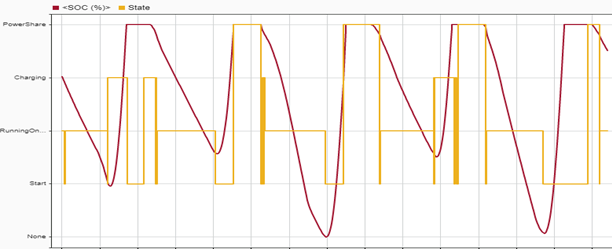
\includegraphics[totalheight=6cm]{Figures/five-day Solar farm SoC v Operation state.png}
	\caption{Five-day Solar farm SoC v Operation state.}
	%	\label{fig:verticalcell}
\end{figure} 

\subsection{Lab results - Unit 2}
\begin{table}[!ht]
	\begin{center}
		\caption{Unit2 - Laboratory setup parameters}
		%\label{tab:table2}
		\begin{tabular}{|p{6cm}|p{8cm}|} % <-- Alignments: 1st column left, 2nd middle and 3rd right, with vertical lines in between
			\hline
			Battery size and capacity	& Nominal voltage: 12V DC \\
			& Capacity: 17Ah\\
			\hline
			Load Size 					& Minimum: 60(W)\\
			& Maximum: 520(W)\\
			\hline
			PV module		 			& None\\
			\hline
		\end{tabular}
	\end{center}
\end{table}

Unit 2 relies on the grid to charge its battery storage, as illustrated in Figure 4.44. The control system maintains grid stability by disconnecting loads when necessary. Due to the limited battery size, the supply sometimes fails to meet demand, causing the unit to be unable to fully power appliances in certain situations. However, the control system prevents the batteries from completely discharging, thereby protecting their health.\par

\begin{figure}[H]
	\centering
	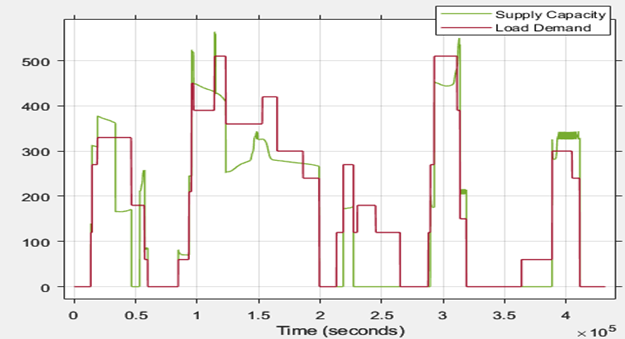
\includegraphics[totalheight=6cm]{Figures/Unit 2 Supply Capacity v Load Demand.png}
	\caption{Unit 2 Supply Capacity v Load Demand.}
	%	\label{fig:verticalcell}
\end{figure} 
Prioritizing grid usage over local storage allows local loads to operate for longer periods. However, due to the limited battery capacity, the local state of charge (SOC) drops quickly, necessitating the control system to switch to grid usage. The comparison between solar farm and local storage SOCs is shown below.\par
\begin{figure}[H]
	\centering
	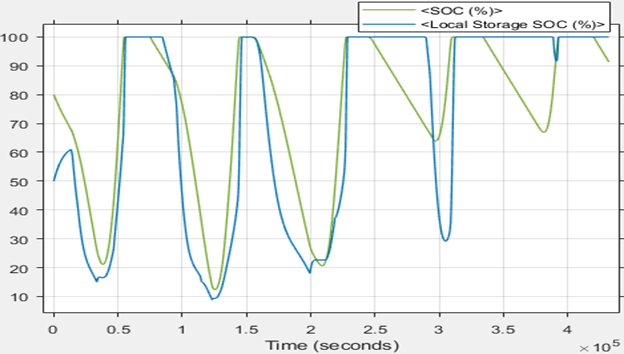
\includegraphics[totalheight=6cm]{Figures/Unit 2 Solar Farm v local storage SoC.png}
	\caption{Unit 2 Solar Farm v local storage SoC}
	%	\label{fig:verticalcell}
\end{figure} 
\subsection{Lab results - Unit 3}
\begin{table}[!ht]
	\begin{center}
		\caption{Unit3 - Laboratory setup parameters}
		%\label{tab:table2}
		\begin{tabular}{|p{6cm}|p{8cm}|} % <-- Alignments: 1st column left, 2nd middle and 3rd right, with vertical lines in between
			\hline
			Battery size and capacity	& None\\
			\hline
			Load Size 					& Minimum: 60(W)\\
			& Maximum: 400(W)\\
			\hline
			PV module		 			& Maximum power: 330(W).\\
										& Vmp: 36.92(V).\\
										& Imp: 8.14(A)\\
			\hline
		\end{tabular}
	\end{center}
\end{table}
Unit 3 is highly dependent on the grid from sunset to sunrise. During this period, loads are significantly limited to conserve power. This dependency highlights the importance of efficient energy management in off-peak hours. By restricting load usage, the system ensures that essential functions can continue without overloading the grid.\par

\begin{figure}[H]
	\centering
	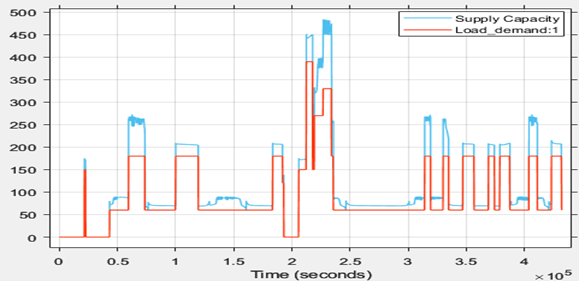
\includegraphics[totalheight=6cm]{Figures/Unit 3 Supply Capacity v Load Demand.png}
	\caption{Unit 3 Supply Capacity v Load Demand}
	%	\label{fig:verticalcell}
\end{figure}

\subsection{Lab results - Unit 4} 
\begin{table}[!ht]
	\begin{center}
		\caption{Unit3 - Laboratory setup parameters}
		%\label{tab:table2}
		\begin{tabular}{|p{6cm}|p{8cm}|} % <-- Alignments: 1st column left, 2nd middle and 3rd right, with vertical lines in between
			\hline
			Battery size and capacity	& None\\
			\hline
			Load Size 					& Minimum: 60(W)\\
			& Maximum: 400(W)\\
			\hline
			PV module		 			& None\\
			\hline
		\end{tabular}
	\end{center}
\end{table}


Unit 4 is entirely dependent on the grid, making it highly sensitive to any major changes in the grid system. This unit underscores the critical importance of maintaining grid stability. It also demonstrates the necessity of self-management; without an Energy Management System (EMS) to control local loads and the absence of local storage and generation capacity, this unit could potentially destabilize the grid.
\begin{figure}[H]
	\centering
	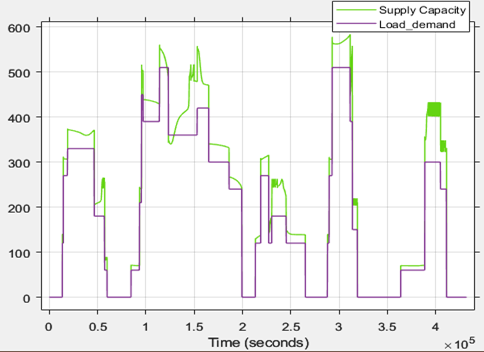
\includegraphics[totalheight=6cm]{Figures/Unit 4 Supply Capacity v Load Demand.png}
	\caption{Unit 4 Supply Capacity v Load Demand}
	%	\label{fig:verticalcell}
\end{figure}
The system optimizes energy use by adjusting to consumption patterns, activating power-saving measures when demand exceeds supply, and extending battery lifespan by preventing over-discharge. Power sharing from solar panels occurs when local battery storage is full, benefiting the grid. In Unit 2, which relies on the grid for charging due to limited battery capacity and no PV module, the control system ensures stability by disconnecting loads as needed and preventing complete battery discharge. Grid usage is prioritized to extend operation times, though the local state of charge drops quickly, requiring a switch to grid power.\par
The laboratory system's responses are similar to the Matlab simulation since the unit's EMS remains consistent; any variations are due to differences in battery capacity and load.











